%%%%%%%%%%%%%%%%%%%%%%%%%%%%%%%%%%%%%%%%%%%%%%%%%%%%%%%%%%%%%%%%%%%
%%% Documento LaTeX 																						%%%
%%%%%%%%%%%%%%%%%%%%%%%%%%%%%%%%%%%%%%%%%%%%%%%%%%%%%%%%%%%%%%%%%%%
% Título:		Capítulo 1
% Autor:  	Ignacio Moreno Doblas
% Fecha:  	2014-02-01
% Versión:	0.5.0
%%%%%%%%%%%%%%%%%%%%%%%%%%%%%%%%%%%%%%%%%%%%%%%%%%%%%%%%%%%%%%%%%%%
\chapterbegin{Introducción teórica}
\label{chp:ManLaTeX}
\minitoc

\begin{sinopsis}
\label{sec:chpltx:sinop}
	
\end{sinopsis}

\section{Acústica}
\label{sec:RuidoAmb}

\subsection{Nivel de presión sonora}

\subsection{Control automático de ganancia (CAG)}

\subsection{Modulación por impulsos codificados}

\subsection{Mapa de calor}

\section{Android}
\label{sec:AndroidIntro}

Android es un sistema operativo, en sus inicios concebido para dispositivos móviles con pantalla táctil, que ha evolucionado en una plataforma que actualmente también engloba relojes inteligentes, televisores, automóviles e incluso electrodomésticos.

Está basado en el núcleo de Linux, sobre el que corre el entorno de ejecución propio de Android (ya sea Dalvik o ART), y este a su vez ejecuta el código de las aplicaciones, escritas mayoritariamente en Java, aunque se permiten extensiones en C/C++

\begin{figure}[h] \centering
    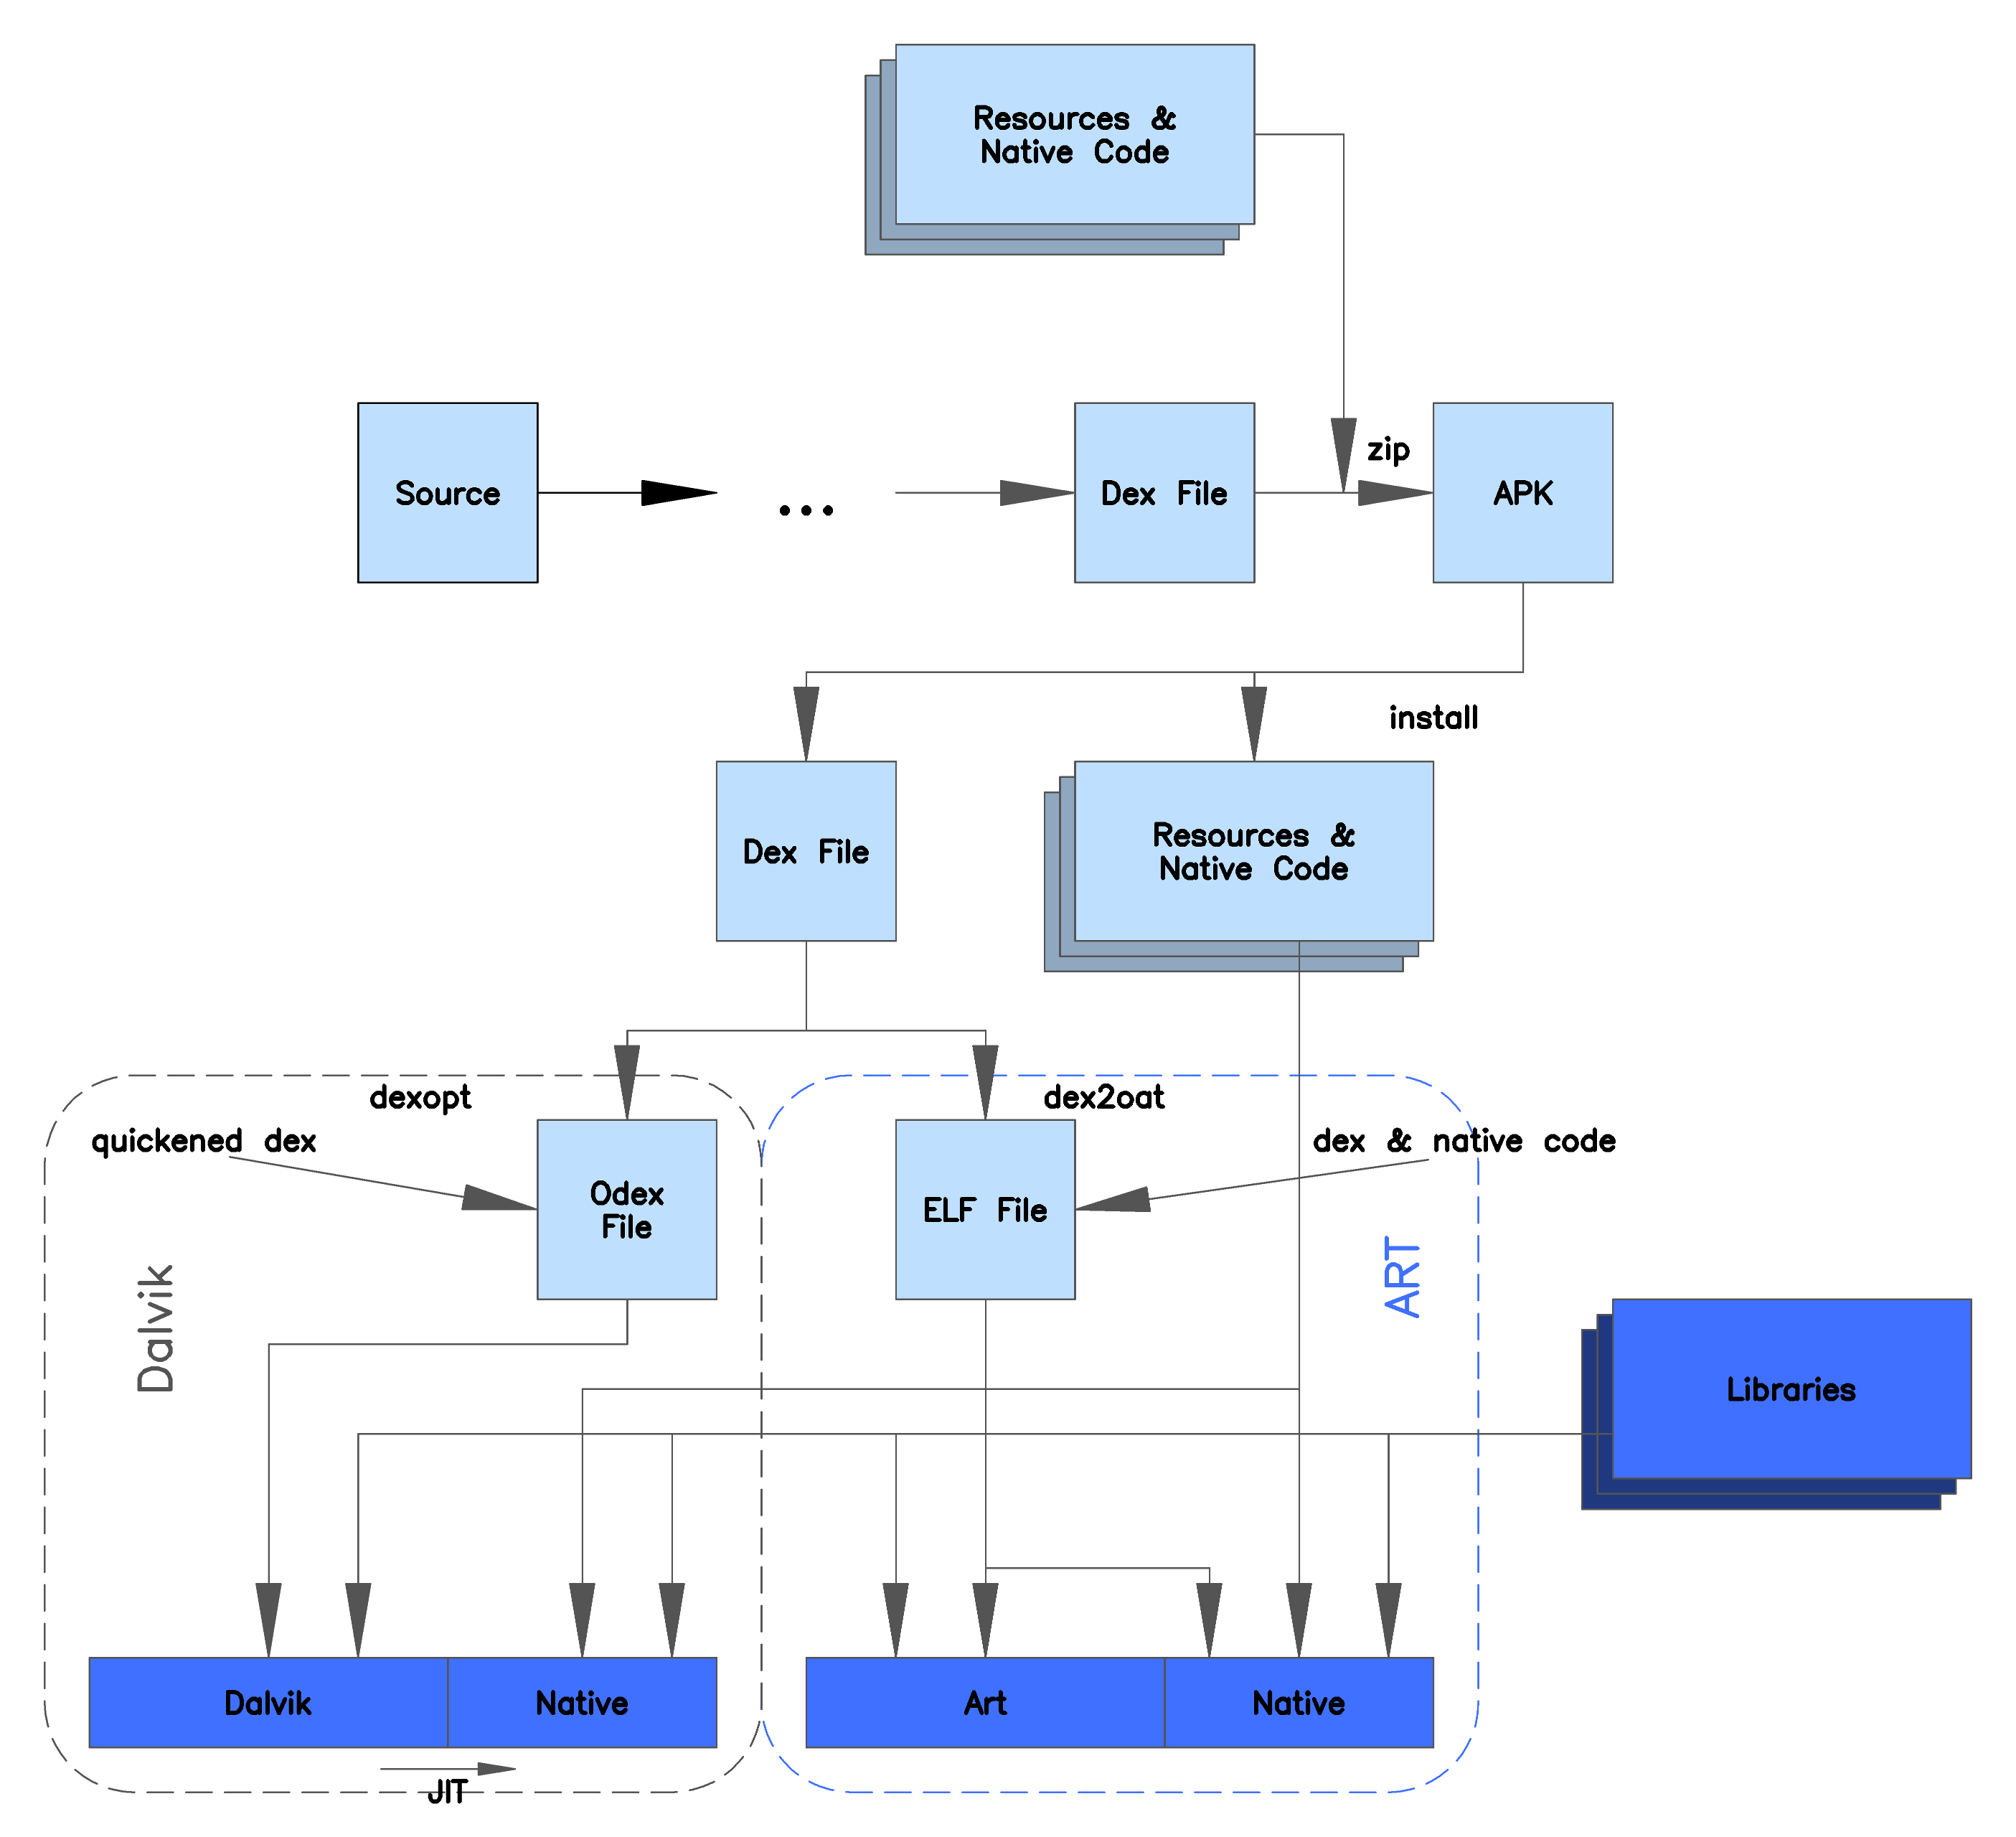
\includegraphics[height=12cm]{graphs/ART_view.png} \caption{Diagrama de la estructura del sistema operativo Android}\label{fig:diagrama:ART}
\end{figure}

\subsection{Interfaz}

La interfaz de usuario por defecto de Android está basada en una manipulación directa, usando entrada táctil con gestos que vagamente corresponden a acciones físicas reales, tales como deslizar, golpear, pellizcar… para manipular objetos en pantalla. Además, la mayoría de dispositivos dispone de un teclado virtual, manipulado de la misma manera. 

La respuesta del sistema a la entrada del usuario está diseñada para ser inmediata y dar una sensación de fluidez, utilizando las capacidades de vibración presentes en la mayoría de los dispositivos para proveer una respuesta háptica (no visual, no auditiva). Adicionalmente, algunas aplicaciones utilizan la información proveída por sensores tales como acelerómetros, giroscopios y sensores de proximidad para responder a interacciones adicionales, como por ejemplo ajustar la orientación de la pantalla cuando el dispositivo se encuentra apaisado o controlar alguna parte de la aplicación basándose en el azimut relativo del dispositivo.

Una parte importante de la interfaz general de Android son las notificaciones, presentes en la barra de estado

\subsection{Componentes de una aplicación}

\subsubsection{Contexto}

Uno de los conceptos más importantes cuando se utiliza la plataforma Android es el contexto, \ttw{Context}. La clase \ttw{Context} en si misma no es más que una interfaz a información global acerca del entorno de una aplicación, y como tal es abstracta. Sin embargo, es importante ser consciente de qué elementos representan un contexto válido y qué elementos no, ya que un contexto permite acceso a recursos y clases específicos de la aplicación, y llamadas al sistema para operaciones a nivel de aplicación, tales como lanzar actividades, emitir mensajes de difusión o recibirlos.

\subsubsection{Actividades}

En android, una actividad (\ttw{Activity}) representa una única cosa concreta que el usuario puede realizar en la aplicación. La mayoría de las actividades interaccionan con el usuario, por tanto la clase \ttw{Activity} se encarga de crear una ventana donde se puedan insertar los componentes de la interfaz de usuario. Aunque las actividades suelen ser vistas por el usuario como ventanas a pantalla completa, también pueden ser usadas en otras múltiples maneras, ya sea como ventanas flotantes, o incrustadas dentro de otra actividad (mediante un \ttw{ActivityGroup})

\subsubsection{Ciclo de vida de una actividad}
Las distintas actividades de las distintas aplicaciones instaladas en el dispositivo Android son gestionadas en forma de una \tit{pila de actividades}.
 
Cuando el sistema Android se inicia, se presenta al usuario una pantalla principal, desde donde puede lanzar varias acciones y aplicaciones. A partir de ahí, cuando una nueva actividad es empezada, se emplaza arriba de la pila y se convierte en la actividad en ejecución. Las actividades previas si las hubiera siempre permanecen por debajo en la pila, y no se traerán al frente hasta que la nueva actividad finalice.

Una actividad tiene cuatro estados básicos:

\begin{description}
    \item[Activa] \hfill \\
     Una actividad está \tit{activa} cuando está presente en primer plano en la pantalla, es decir, arriba de la pila. También se puede decir que la actividad está \tit{En ejecución}.

    \item[Pausada] \hfill \\
    Si una actividad ha perdido el foco (ha dejado de estar en primer plano) pero todavía es visible, es decir, si una nueva actividad que no ocupa la totalidad de la pantalla o es transparente obtiene el primer plano, se encuentra \tit{pausada}. Una actividad pausada se conserva completamente íntegra (mantiene todos los estados y se mantiene suscrita al gestor de ventanas) pero puede ser matada por el sistema en condiciones extremas de baja memoria disponible.

    \item[Parada] \hfill \\
    Si una actividad se encuentra oculta por completo, el sistema la deja \tit{parada}. Mantiene estados e información de los miembros, pero sin embargo al no ser visible por el usuario es más probable que el sistema se deshaga de ella para liberar recursos cuando hagan falta.
    
    \item[Muerta] \hfill \\
    Cuando el sistema decide mover la actividad fuera de memoria, puede o bien finalizarla o matar el proceso. Cuando sea mostrada de nuevo al usuario, debe ser completamente reiniciada y restaurada a su estado previo.
    
\end{description}

\begin{figure}[h] \centering
    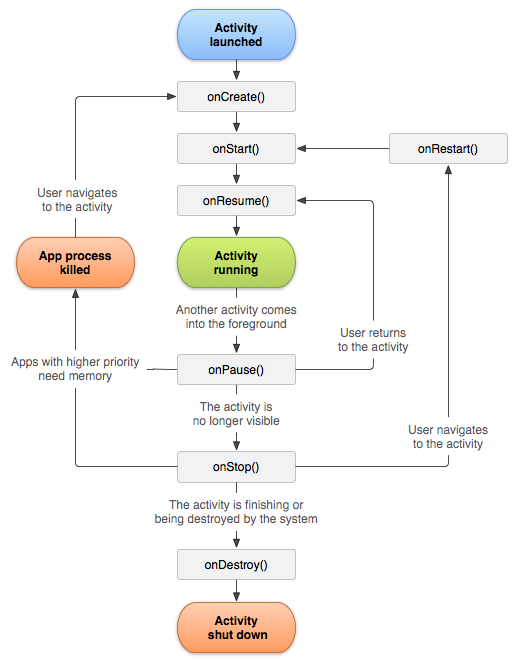
\includegraphics[height=12cm]{graphs/activity_lifecycle.png} \caption{Diagrama del ciclo de vida de una actividad en Android. Tomado de \cite{androiddevguide}.}\label{fig:diagrama:ActivityLifecycle}
\end{figure}

\subsubsection{Servicios}

Un Servicio (\ttw{Service}) es un componente de la aplicación que puede realizar tareas de larga duración en segundo plano y no provee ninguna interfaz de usuario. Otro componente de la aplicación puede iniciar un servicio y este continuará en marcha en segundo plano, incluso si el usuario cambia a otra aplicación distinta. Además, un componente puede adherirse (\ttw{bind}) a un servicio para interacutar con él, e incluso realizar comunicación inter-procesos (IPC por sus siglas en inglés, Inter-Process Communication). Por ejemplo, un servicio puede manejar llamadas de red, reproducir música, realizar operaciones en el sistema de archivos, todo en segundo plano.

Un servicio puede tomar dos estados:

\begin{description}
    \item[Started] \hfill \\
    Un servicio está en estado \ttw{Started} (empezado) cuando un componente de la aplicación, por ejemplo una actividad, lo empieza llamando al método \ttw{startService()}. Una vez empezado de esta manera, un servicio puede continuar en segundo plano de manera indefinida, incluso si el componente que lo empezó ha sido destruído. Normalmente, suelen ser servicios que realizan una única operación y no devuelven ningún resultado. Por ejemplo, puede descargar o subir un archivo en la red. Cuando la operación ha sido completada, el servicio debe pararse a si mismo.
    \item[Bound] \hfill \\
    Un servicio está en estado \ttw{Bound} (adherido) cuando un componente de la aplicación se adhiere a él llamando al método \ttw{bindService()}. Un servicio adherido ofrece una interfaz servidor-cliente que permite a los componentes interaccionar con el servicio, mandar peticiones, obtener resultados, e incluso hacerlo entre distintos procesos mediante comunicación inter-proceso (IPC). Un servicio adherido solamente es activo durante el tiempo que otro componente esté adherido a él. Varios componentes pueden estar adheridos en un momento dado al servicio, pero cuando todos se desadhieren del servicio, el servicio es destruído.

\end{description}

\begin{figure}[h] \centering
    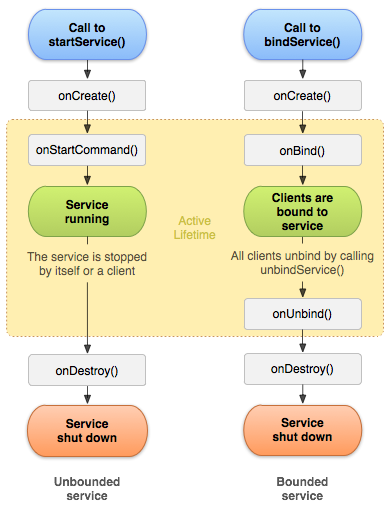
\includegraphics[height=12cm]{graphs/service_lifecycle.png} \caption{Diagrama del ciclo de vida de un servicio. Tomado de \cite{androiddevguide}}\label{fig:diagrama:ServiceLifecycle}
\end{figure}

Hay que tener cuidado, dado que un servicio corre en el hilo principal de ejecución del proceso que lo llama, a no ser que se especifique lo contrario. Esto implica que, si el servicio va a realizar alguna tarea intensiva en CPU, o alguna operación bloqueante, se debe de crear un nuevo hilo de ejecución dentro del servicio para ese propósito. De no hacerlo, se corre el riesgo de que la aplicación deje de responder y sea matada por el sistema operativo.


\subsection{Vistas}

La interfaz gráfica de usuario en una aplicación Android está construida usando una jerarquía de vistas, objetos de la clase \ttw{View}, y grupos de vistas, objetos de la clase \ttw{ViewGroup}. Los objetos \ttw{View} suelen ser artilugios (widgets) de la interfaz de usuario, tales como botones o campos de texto, y los objetos \ttw{ViewGroup} son contenedores invisibles que definen cómo se posicionan las vistas que dependen de ellos, por ejemplo dispuestas en forma de rejilla o lista vertical.

Android provee un vocabulario XML que se corresponde con las subclases de \ttw{View} y \ttw{ViewGroup}, y permite definir la interfaz de usuario en XML usando una jerarquía de elementos de interfaz de usuario.

\subsection{Procesos e hilos de ejecución}

En sistemas operativos, son básicos los conceptos de proceso e hilo de ejecución. En Android, el sistema operativo comienza un nuevo proceso Linux por cada primer componente de cada aplicación, con un único hilo de ejecución. Por defecto, todos los componentes de la misma aplicación corren en los mismos proceso e hilo de ejecución, el hilo principal de ejecución (\tit{main thread} en inglés). 

En caso de que un componente de una aplicación sea inicializado, y ya exista un proceso para dicha aplicación en el sistema que otro componente de la misma aplicación ha inicializado, el nuevo componente se inicializa dentro del proceso roiginal y usa el mismo hilo de ejecución. Sin embargo, se puede configurar una aplicación de manera que diferentes componentes corran en procesos separados, y siempre se pueden crear hilos de ejecución adicionales para cualquier proceso.

\subsubsection{Procesos}

Como ya ha sido expuesto anteriormente, por defecto todos los componentes de la misma aplicación corren en el mismo proceso, y la mayoría de las aplicacones no deberían de cambiarlo. Sin embargo, es posible controlar qué proceso pertenece a qué componente de ser necesario.

El sistema operativo puede decidir apagar un proceso, cuando la cantidad de memoria disponible sea baja y haya requerimiento de ella por otro proceso que sirva de manera más inmediata al usuario. En este caso, los componentes dentro de dicho proceso que es apagado, son destruidos. Cuando estos componentes sean necesarios de nuevo, un nuevo proceso será comenzado por el sistema operativo para ello.

\subsubsection{Hilos de ejecución}

Previamente se ha mencionado que todos los componentes de la misma aplicación corren en el mismo hilo de ejecución, el hilo principal de ejecución o \tit{main thread}. Éste hilo es de suma importancia, dado que carga con la responsabilidad de despachar los eventos al widget de la interfaz de usuario que sea pertinente, incluyendo los eventos de dibujado en pantalla. Es también el hilo de ejecución en el que la aplicación interactúa con los componentes básicos de interfaz de usuario de Android, también conocidos como \tit{Android UI toolkit} (ubicados dentro de los paquetes java \ttw{android.widget} y \ttw{android.view}). Por todo esto, no es extraño encontrar denominado este hilo de ejecución como el hilo de la interfaz de usuario, o \tit{UI Thread}.

Dado que todos los componentes que corren en el mismo porceso son instanciados en el hilo de ejecución principal, las llamadas del sistema operativo a cada componente son despachadas desde dicho hilo. En consecuencia, todos los métodos que responden a retrollamadas del sistema (\tit{system callbacks}), como por ejemplo para indicar que una tecla ha sido pulsada, siempre corren en el hilo principal de ejecución del proceso.

Cuando el usuario toca un botón en la pantalla, el hilo principal de la aplicación despacha el evento de toque al widget pertinente, que reacciona cambiando su estado a presionado y manda una petición de invalidación a la cola de eventos. El hilo de ejecución principal entonces desencola la petición y notifica al widget qque debe de redibujarse.

Cuando una aplicación realiza trabajo intensivo en respuesta a una interacción del usuario, el modelo de hilo de ejecución único puede resultar en una falta de rendimiento. Concretamente, de suceder todo el procesamiento en el hilo principal de ejecución e iniciar tareas de larga ejecución tales como acceso a red o consultas a bases de datos, resultará en un bloqueo completo de la interfaz de usuario y su correspondiente hilo principal. Cuando el hilo de ejecución está bloqueado, no se pueden despachar eventos, eventos de dibujado en pantalla incluidos. Desde el punto de vista del usuario, esto se traduce en una aplicación que parece colgarse. En peores casos, en los que el hilo principal de ejecución está bloqueado por más de unos cuantos segundos (cinco segundos en la actualidad) el sistema operativo entrará en acción y mostrará una pantalla explicando que la aplicación ha dejado de responder, y matará la aplicación bloqueada. 

 Para evitar dicha penalización en el rendimiento, deben usarse hilos de ejecución alternativos para toda tarea que bloquee la ejecución o sea de alta carga procedural.

\subsection{Servicios de Google Play}

\subsection{Manejo de archivos}

\chapterend{}